\documentclass{standalone}
\usepackage{amsmath}
\usepackage{tikz}
\usetikzlibrary{arrows, calc, backgrounds, positioning}

\newcommand\dataline[4]{
    \draw [line width=#1 mm] (#2) to [#4] (#3);
}

\tikzstyle{background} = [fill=green!5!white,draw=green!75!black,very thick]
\tikzstyle{titlebox} = [fill=green!75!black,text=black,rounded corners]

\tikzstyle{disk}       = [rectangle,draw=black!50,fill=black!20,align=left,rotate=90]
\tikzstyle{controller} = [rectangle,draw=red!80,fill=red!20,align=left]
\tikzstyle{network}    = [rectangle,draw=blue!80,fill=blue!20,align=left]
\tikzstyle{switch}     = [rectangle,draw=green!80,fill=green!20,align=left]

% Network latency is 0.004 ms
%  Disk   latency is 4     ms

% If the sep between NIC and switch is 2cm, then using a log scale, the
% disks are (2 cm) * log(4 / 0.004) = 13.8 cm below the RAID controller

\begin{document}
    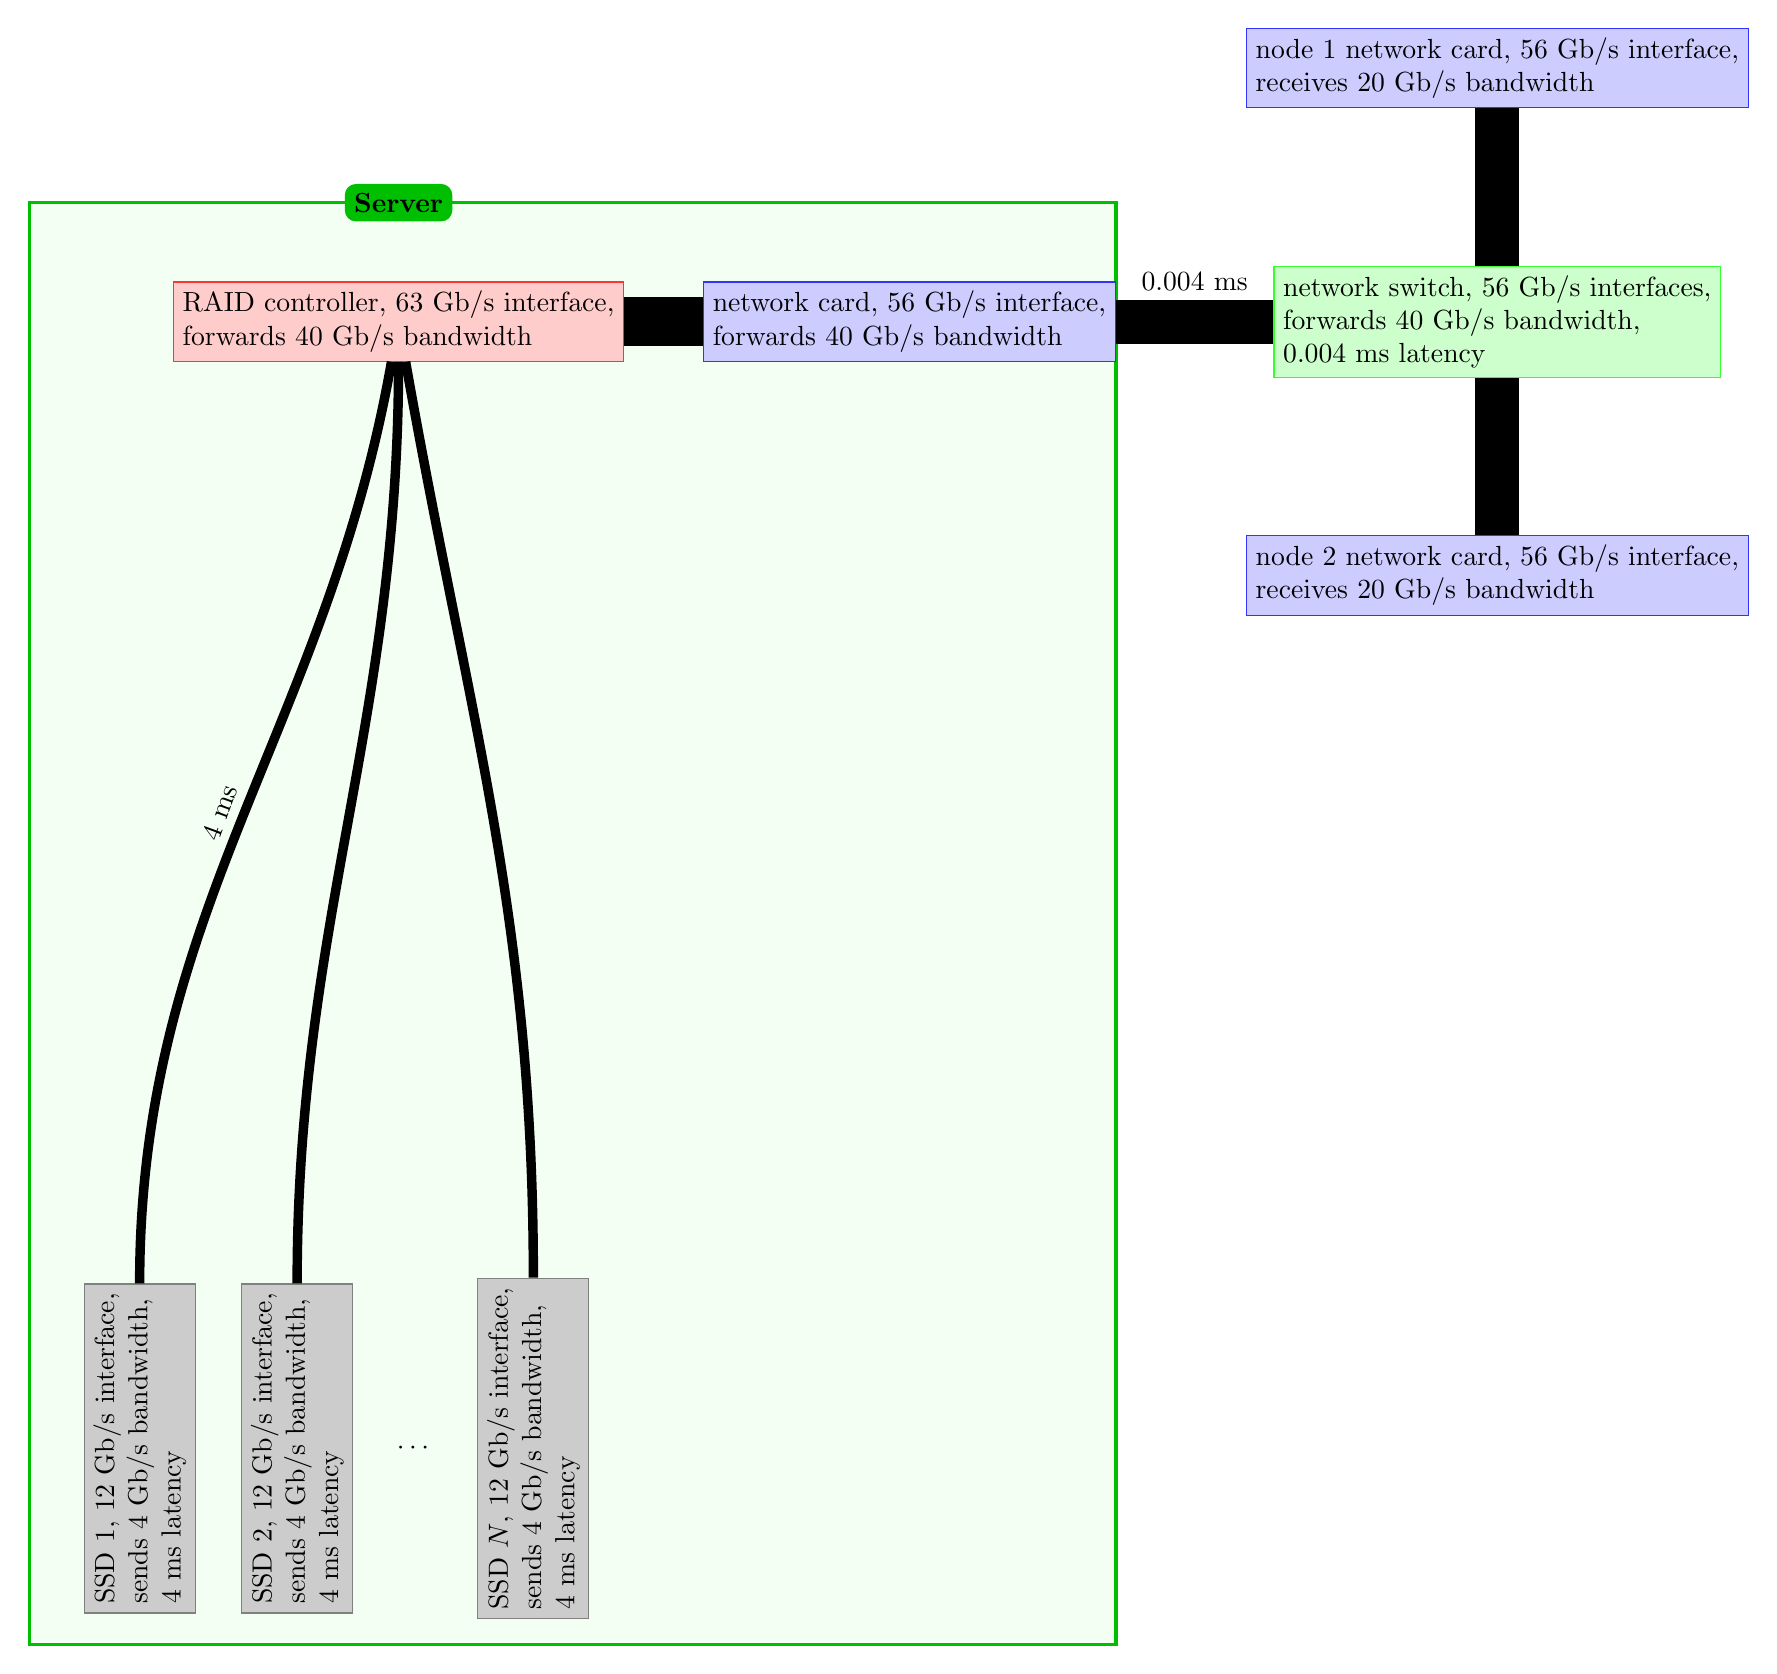
\begin{tikzpicture}
        \node[controller]           (raid)                                           {RAID controller, 63 Gb/s interface,\\ forwards 40 Gb/s bandwidth};
        \node[disk,anchor=north]    (disk 1)     at ($(raid.south)+(-4cm, -13.8cm)$) {SSD 1, 12 Gb/s interface,\\ sends 4 Gb/s bandwidth,\\ 4 ms latency};
        \node[disk]                 (disk 2)     at ($(disk 1) + (2cm, 0)$)          {SSD 2, 12 Gb/s interface,\\ sends 4 Gb/s bandwidth,\\ 4 ms latency};
        \node                       (dots)       at ($(disk 2) + (1.5cm, 0)$)        {$\cdots$};
        \node[disk]                 (disk N)     at ($(dots) + (+1.5cm, 0)$)         {SSD $N$, 12 Gb/s interface,\\ sends 4 Gb/s bandwidth,\\ 4 ms latency};
        \node[network]              (nic)        [right=of raid]                     {network card, 56 Gb/s interface,\\ forwards 40 Gb/s bandwidth};
        \node[switch,anchor=west]   (switch)     at ($(nic.east) + (2cm, 0)$)        {network switch, 56 Gb/s interfaces,\\ forwards 40 Gb/s bandwidth,\\ 0.004 ms latency};
        \node[network,anchor=south] (node 1 nic) at ($(switch.north)+(0, 2cm)$)      {node 1 network card, 56 Gb/s interface,\\ receives 20 Gb/s bandwidth};
        \node[network,anchor=north] (node 2 nic) at ($(switch.south)+(0,-2cm)$)      {node 2 network card, 56 Gb/s interface,\\ receives 20 Gb/s bandwidth};

        \draw[line width=1.2mm, out=90, in=260] (disk 1.east) to node[above,rotate=70] {4 ms} (raid);
        \dataline{1.2}{disk 2.east}{raid}{out=90,in=270}
        \dataline{1.2}{disk N.east}{raid}{out=90,in=280}
        \dataline{6.3}{raid}{nic}{}
        \draw[line width=5.6mm] (nic) to node[above]{0.004 ms} (switch);
        \dataline{5.6}{switch}{node 1 nic}{}
        \dataline{5.6}{switch}{node 2 nic}{}

        \node[titlebox] (server) at ($(raid.north)+(0cm, 1cm)$) {\textbf{Server}};

        \begin{pgfonlayer}{background}
		    \draw [background] ($(server.west)+(-4cm, 0)$) rectangle ($(nic.east)+(0cm, -16.8cm)$);
        \end{pgfonlayer}
    \end{tikzpicture}
\end{document}
